%%%% Weekly Report Information %%%%
\newcommand{\handoutName}{Weekly report}
\newcommand{\handoutdate}{\today}
%\newcommand{\duedate}{}
% Header template used for Weekly Reports
\documentclass[11pt,twoside]{article}

\setlength{\oddsidemargin}{0pt}
\setlength{\evensidemargin}{0pt}
\setlength{\textwidth}{6.5in}
\setlength{\topmargin}{0in}
\setlength{\textheight}{8.5in}
\setlength{\voffset}{0in}

\providecommand{\titlesize}{small}


\usepackage{graphicx}
%\usepackage{subfigure}
\usepackage{palatino}
%\usepackage{cmbright}
\newcommand{\myMargin}{1.00in}
%\usepackage[pdftex]{hyperref}
\usepackage[small,bf]{caption}
%\usepackage{amsmath}
\usepackage[usenames,dvipsnames]{color}
\usepackage{fancyhdr}
\pagestyle{fancy}
\usepackage{datetime}
\usepackage{fancyvrb}
\usepackage{color}
\usepackage[\titlesize, compact]{titlesec}
\usepackage{multicol}
\usepackage{enumitem}
\usepackage{pdfpages}
\usepackage{mdwlist}
\usepackage{caption}
\usepackage{subcaption}
\usepackage{hyperref}
\usepackage[cmex10]{amsmath}
\usepackage{algorithmicx}
\usepackage[ruled]{algorithm}
\usepackage{algpseudocode}
\renewcommand\labelenumi{\textbf{\theenumi) }}
\newcommand\algorithmicinput{\textbf{Input:}}
%\newcommand\INPUT{\item[\algorithmicinput]}
\newcommand\algorithmicassume{\textbf{Assume:}}
%\newcommand\ASSUME{\item[\algorithmicassume]}

\newdateformat{dashdate}{\THEYEAR-\twodigit{\THEMONTH}-\twodigit{\THEDAY}}
\def\Tiny{\fontsize{3pt}{3pt}\selectfont}

\providecommand{\handoutName}{Handout title}
\providecommand{\handoutdate}{Handout date}
\providecommand{\duedate}{}

\lhead{Meeting with Prof. Becker\\
Spring, 2017}
\chead{}
\rhead{ Shiva Shahrokhi\\
\handoutdate }
\lfoot{}
\cfoot{\thepage}
\rfoot{\dashdate \Tiny \textcolor{Gray}{\today}}
\renewcommand{\headrulewidth}{0.4pt}
\renewcommand{\footrulewidth}{0.4pt}

\begin{document}

\vspace{0.60in}
\begin{center}
{\Large\textbf{\handoutName}}\\
\vspace{0.03in}
\textbf{\duedate}\\
\end{center}

\newcommand{\todo}[1]{
  \textcolor{Red}{
    \begin{tabular}{|c|}
      \hline
      \em \large \bfseries todo: \normalfont \normalsize #1 \\
      \hline
    \end{tabular}}
}


\section{My \emph{Objectives} this week}
\begin{itemize}
\item I want to implement the partitioning part with map. I have to write an algorithm for that and load that.
\item I hope to be able to finish at least 4 more full experiments and also write all the missing part of the paper.
\item I would start the torque control journal paper with Mable and Lillian, I want to start with the pure torque control task this week and write the code for that.
\end{itemize}



\section{My \emph{Accomplishments} this week}


\begin{itemize}
\item Wrote an automatic torquecontroller which finds the object, understands its orientation and push it.
\item We discussed together about the algorithm of partitioning the map.
So the algorithm is this:\\
We learned from humans that they would ignore the robots that are not on the path of the robots. In our previous work we had this problem that when the robots were separated, and they were in variance control mode, they would get stuck and our algorithm failed. In this work we present an algorithm to make sure that the swarm will not get stuck at any point. First we make the whole map, all the obstacles are pink, and we detect them with our vision system. For simplicity assume that all the obstacles are lines. When an obstacle is detected, it has one or two end points and also its orientation is detected by processing of the snapshot of the webcam. Any of the ending points is a potential for having a big region. Without loss of generality, assume that all the obstacles are attached from one point to the walls. For the other ending point, draw a line until it intersects another obstacle. This cause the map to divide into the regions made by those lines. We call these regions our main regions. There are two states that the object could be in. It starts in the ``main region" state until it hits a boundary line. If it passes a boundary line, it will go to the ``transferring" region state. In this state, we have two temporary lines which each one is in one of the main regions. We consider this area as transferring region. If the object passes those temporary lines, it will go again to the ``main region" state. In each region the algorithm will consider the robots inside that region only. Therefore, if some of the robots were behind, they would not be considered for mean and variance and the swarm would not get stuck.

\begin{figure}[h]
\begin{center}
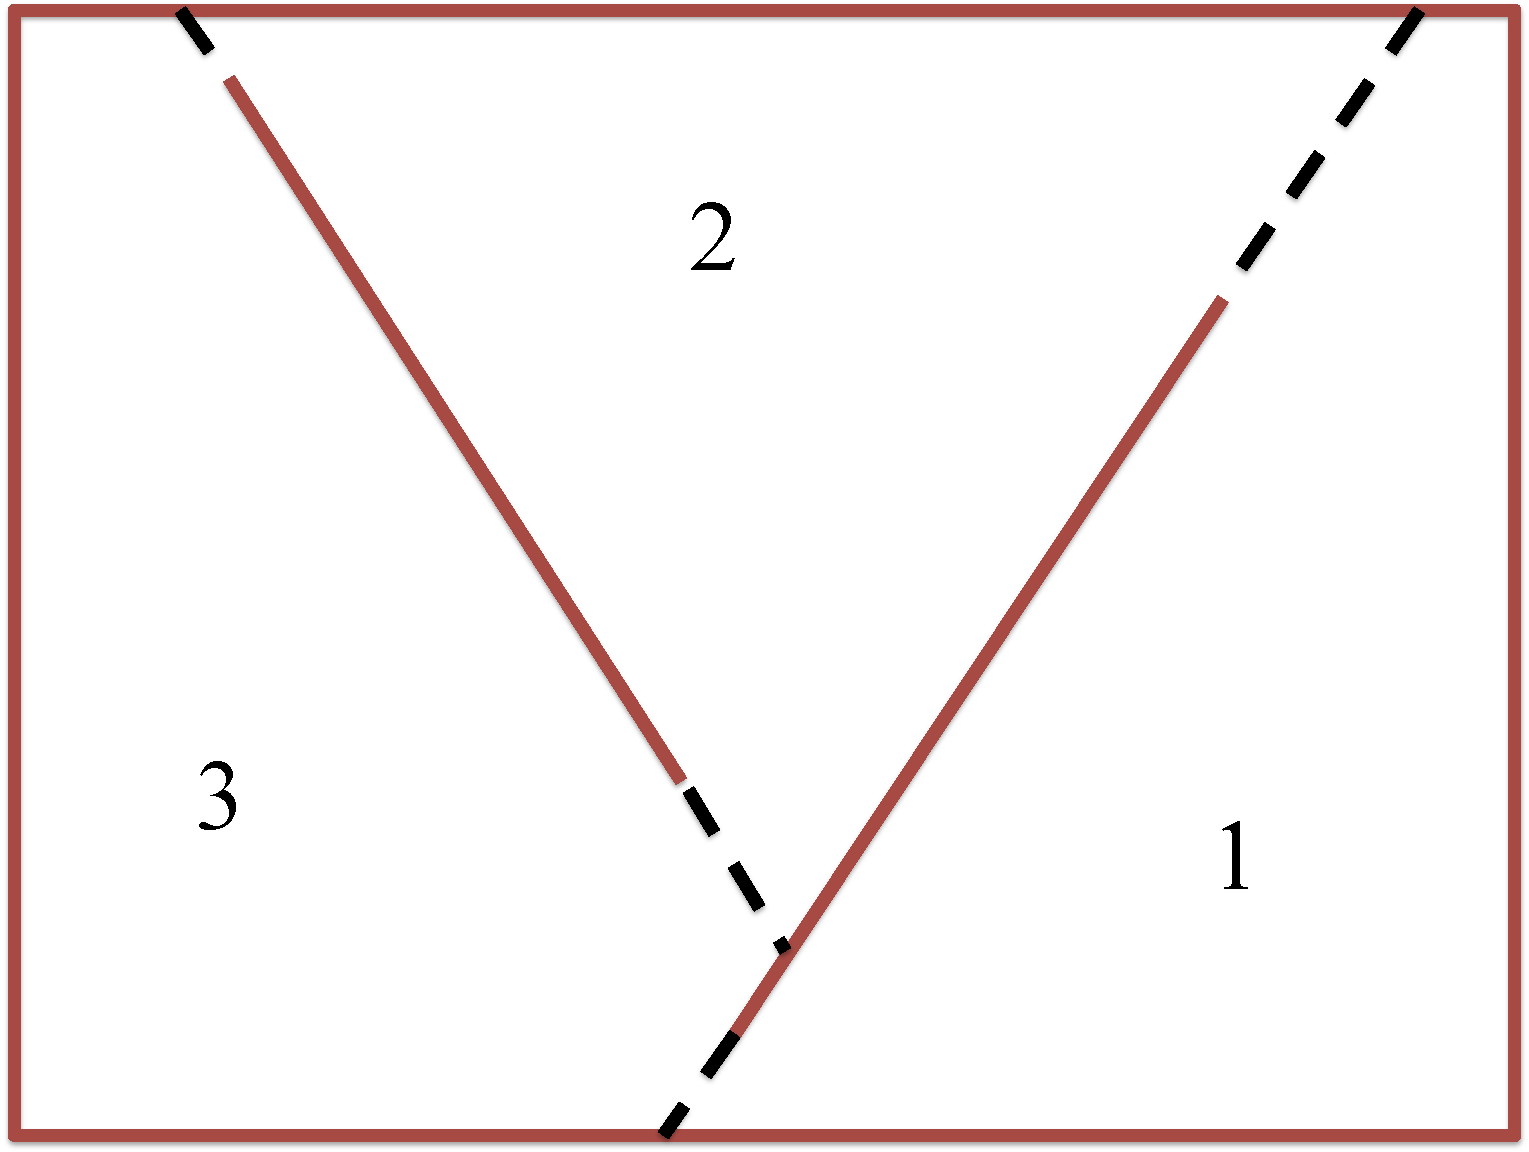
\includegraphics[width=5cm]{pictures/pdf/Regions.pdf}
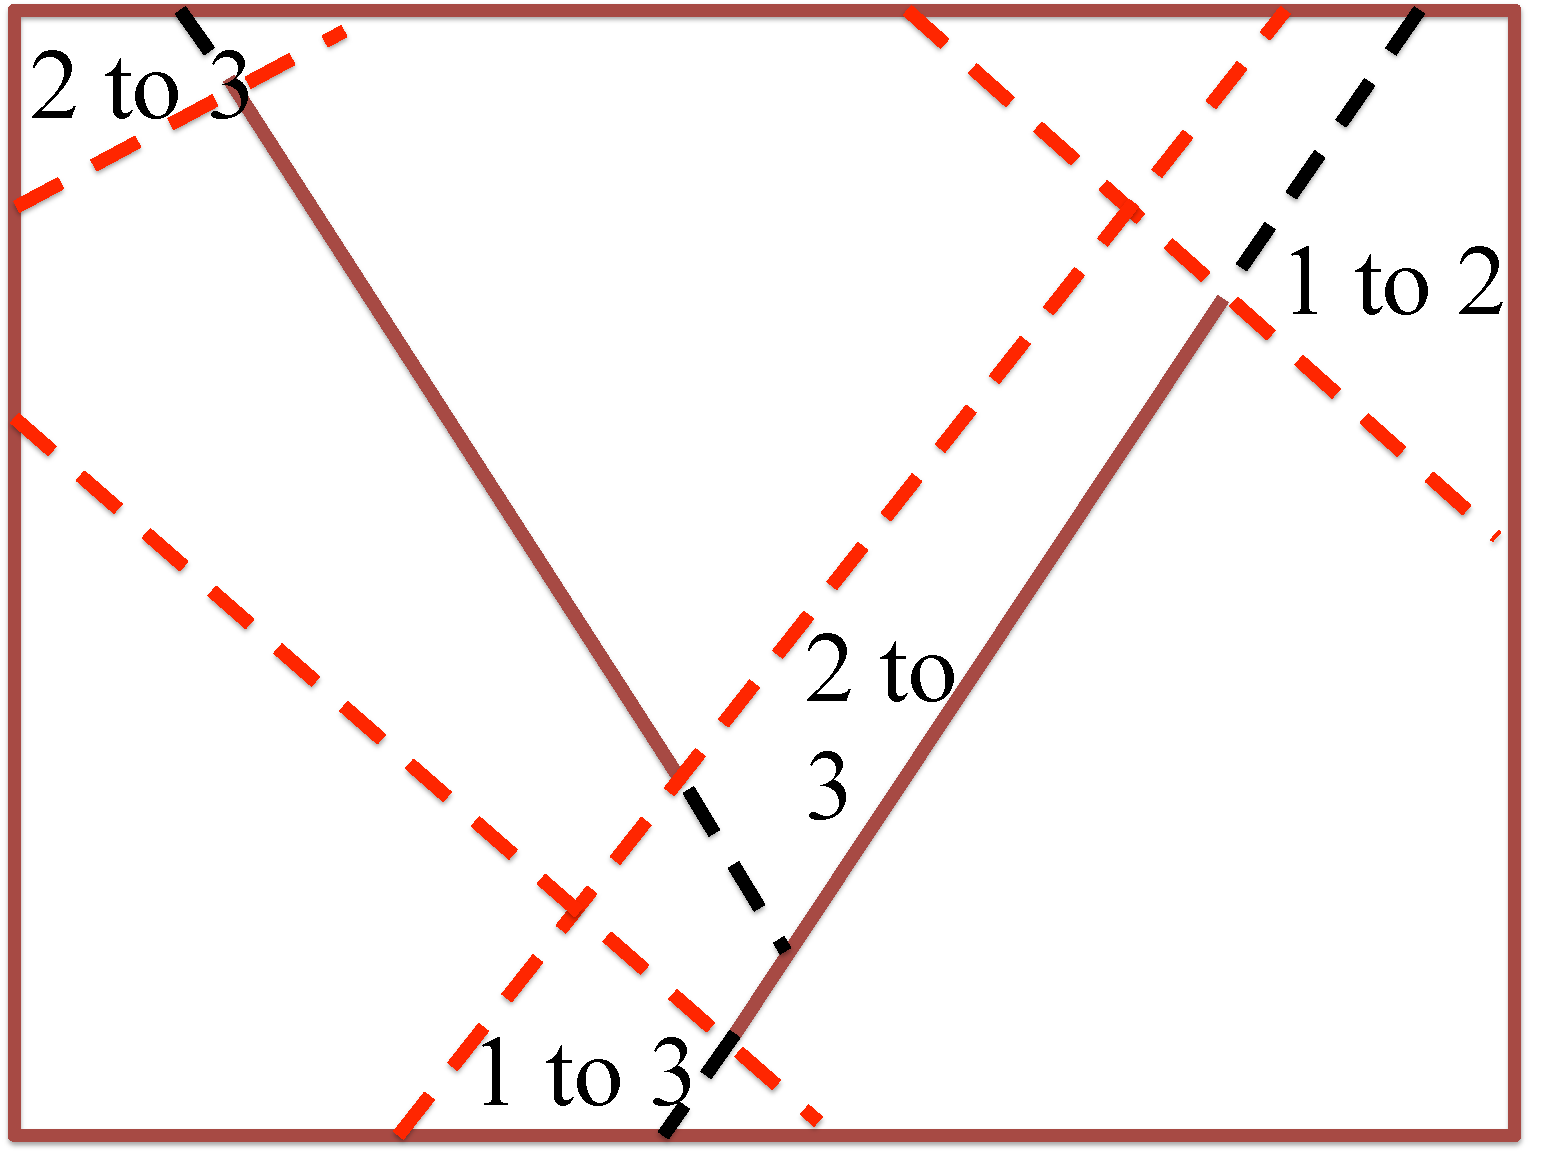
\includegraphics[width=5cm]{pictures/pdf/TransferRegions.pdf}
\caption{An example of having three arbitrary straight obstacles. Left is how the main regions are detected, and right is the transferring regions.}
\end{center}
\end{figure}

\item I wrote the pure torque control challenge in matlab. it is now COMPLETELY autonomous. It sees the pink object, understands its orientation, and you can set different CLs to determine where the goal should be. 
\item Mahek made a light long rectangle with 3D printer. We tested torqueControl using that and got some data, these are the very first datas, I would get the better data and share that with you. There is a small bug for the orientation determining, that at exactly 90 degrees it will change its sign. That is why it starts from -90 degrees and jumps to 90 degrees. It seems to me that because we are not controlling them exactly to the point that they should go, they look really the same. 
\begin{figure}[h]
\begin{center}
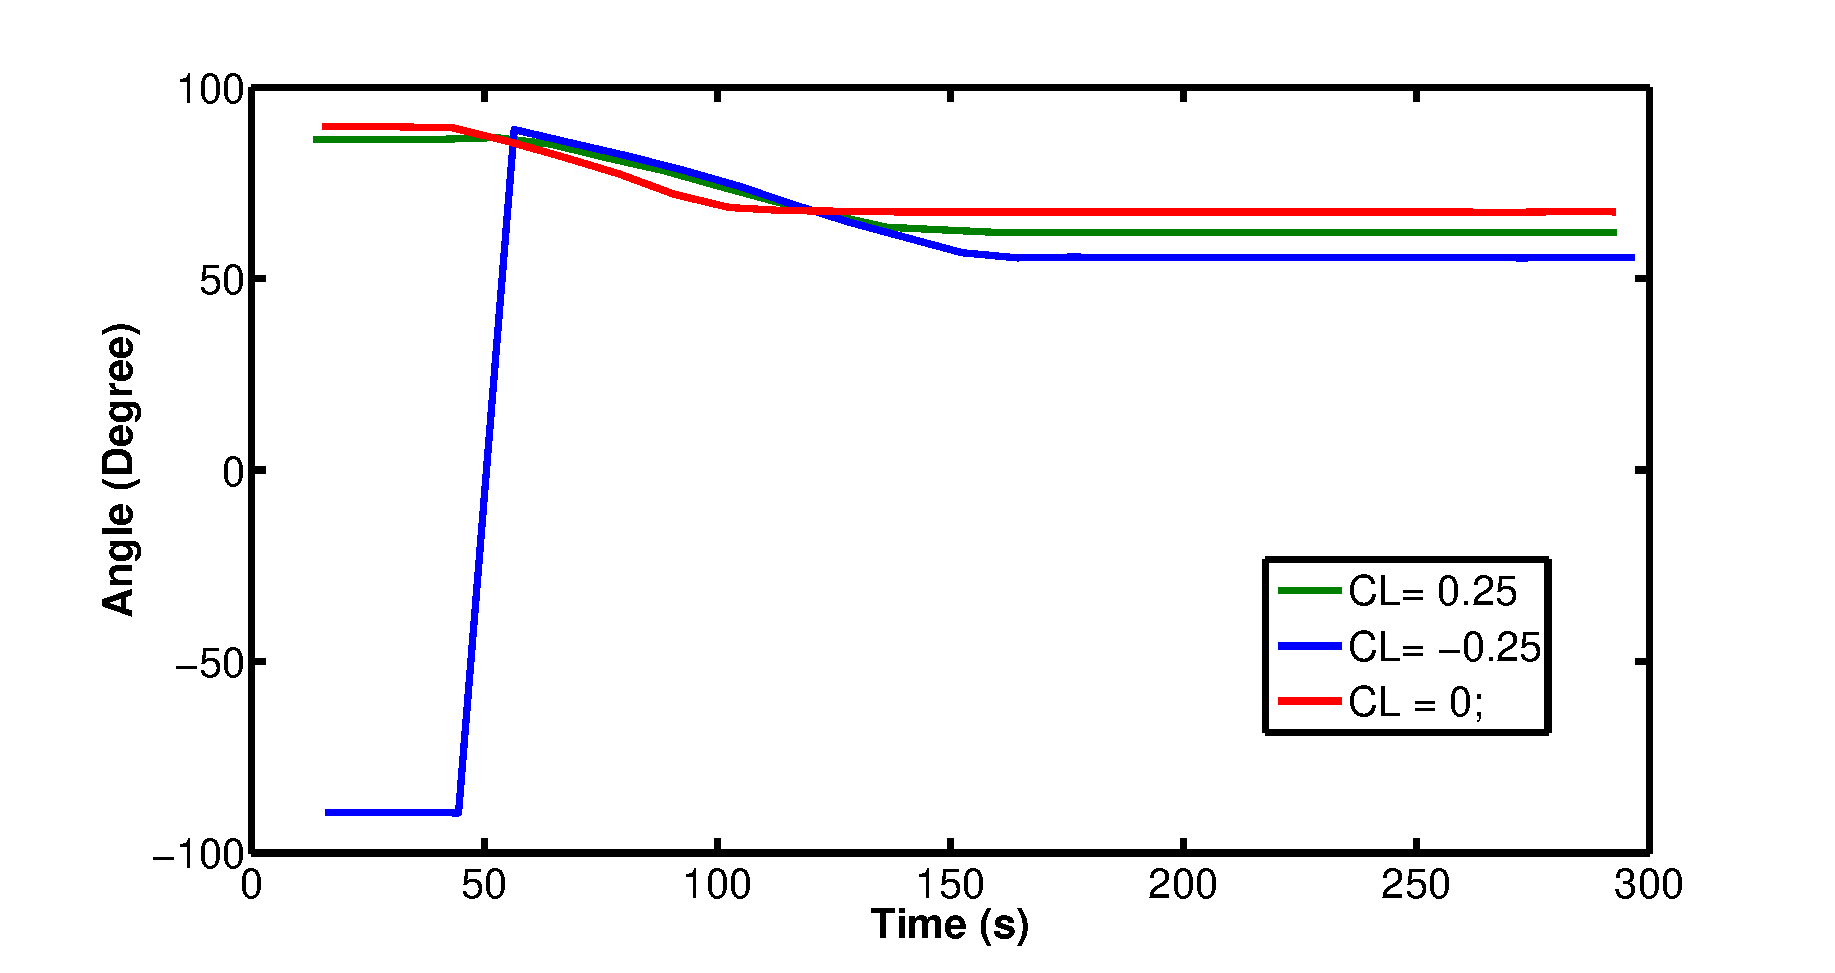
\includegraphics[width=9cm]{TorqueControlResult}
\caption{Three different CLs to find the best. I have to redo these experiments, but I wanted to show how they look.}
\end{center}
\end{figure}
\item I taught Mahek how to use the laser cutter.
\end{itemize}


\section{My \emph{Plan} for next week}

\begin{itemize}
\item I want to implement the partitioning part with map. And test that idea.
\item I would finish the pure torque control experiment and finalize its plots.
\end{itemize}

\subsection{Meeting with Dr. Becker  }

\begin{itemize}
\item I need to talk about the case reviews.
\item I need to talk about our team.
\item I want your feedback on the algorithm.
\end{itemize}

\end{document}
